\documentclass[t]{beamer}
\usetheme[deutsch]{KIT}
\setbeamercovered{transparent}
\setbeamertemplate{navigation symbols}{}

\KITfoot{Tutoriumsmaterial von Alexander Kwiatkowski, Michael Vollmer und Matthias Holoch \hspace{2.5cm} Basierend auf den Folien von Simon Stroh und Moritz v. Looz}
\usepackage[utf8]{inputenc}
\usepackage{amsmath}
\usepackage{ifthen}
\usepackage{amssymb}
\usepackage{tikz}
\usepackage{ngerman}
\usepackage[normalem]{ulem}
\usetikzlibrary{automata}
\usenavigationsymbols


\title{Theoretische Grundlagen der Informatik}
\subtitle{Tutorium}
\author{Alexander Kwiatkowski, Michael Vollmer und Matthias Holoch}

\institute[IKS]{Institut für Kryptographie und Sicherheit}

\TitleImage[height=\titleimageht]{images/tmaschine.png}

\newcommand{\N}{\ensuremath{\mathbb{N}}}
\newcommand{\M}{\ensuremath{\mathcal{M}}}
\newcommand{\classP}{\ensuremath{\mathcal{P}}}
\newcommand{\classNP}{\ensuremath{\mathcal{NP}}}
\newcommand{\co}{\ensuremath{\mathsf{co\text{-}}}}
\newcommand{\pot}{\ensuremath{\mathcal{P}}}
\newcommand{\abs}[1]{\ensuremath{\left\vert #1 \right\vert}}
\newcommand{\menge}[2]{\ensuremath{\left\lbrace #1 \,\middle\vert\, #2 \right\rbrace}}
\newcommand{\ducttape}[1]{\vspace{#1}}
\newcommand{\neglit}[1]{\overline{#1\vphantom{x^a}}}
\newcommand{\recipe}{\raisebox{-.3cm}{
\includegraphics[scale=.15]{images/chefs-cap.png}}\hspace{0.2cm}}
\newcommand{\opt}[1]{\ensuremath{\text{OPT}(#1)}}
\newcommand{\A}[1]{\ensuremath{\mathcal{A}(#1)}}
\renewcommand{\O}[1]{\ensuremath{\mathcal{O}(#1)}}
\newcommand{\msout}[1]{\text{\sout{\ensuremath{#1}}}}

\newcommand{\invincible}{\setbeamercovered{invisible}} %  "Yesss! I am invincible!!" (Boris Grishenko)
\newcommand{\vincible}{\setbeamercovered{transparent}}
\renewcommand{\solution}[1]{\invincible \pause #1 \vincible}
\newcommand{\micropause}{\\[8pt]}

% \@ifundefined{tikzset}{}{\tikzset{initial text=}} % Text "start" bei Startknoten unterdrücken
\tikzstyle{every node}=[thick]
\tikzstyle{every line}=[thick]

\newcommand{\tutnr}[1]{
  \subtitle{Tutorium #1}
	\begin{frame}
		\maketitle
	\end{frame}
}

\newcommand{\uebnr}[1]{
  \subtitle{Anmerkungen zum #1. Übungsblatt}
	\begin{frame}
		\maketitle
	\end{frame}
}

\begin{document}

\newcommand{\start}[3]
{
  \draw (#1*2,#2*2) node{$#3$};
  \draw (#1*2,#2*2) circle(0.4cm);
  \draw [->] (#1*2-0.9,#2) -- (#1*2-0.4,#2);
}
\newcommand{\final}[3]
{
  \draw (#1*2,#2*2) node{$#3$};
  \draw (#1*2,#2*2) circle(0.4cm);
  \draw (#1*2,#2*2) circle(0.32cm);
}
\newcommand{\startfinal}[3]
{
  \draw (#1*2,#2*2) node{$#3$};
  \draw (#1*2,#2*2) circle(0.4cm);
  \draw (#1*2,#2*2) circle(0.32cm);
  \draw [->] (#1*2-0.9,#2) -- (#1*2-0.4,#2);
}
\newcommand{\state}[3]
{
  \draw (#1*2,#2*2) node{$#3$};
  \draw (#1*2,#2*2) circle(0.4cm);
}
\newcommand{\tol}[4]
{
  \draw (#1+#3,#2*2) node[above]{$#4$};
  \draw [->] (#1*2-0.4,#2*2) -- (#3*2+0.4,#2*2);
}
\newcommand{\tor}[4]
{
  \draw (#1+#3,#2*2) node[above]{$#4$};
  \draw [->] (#1*2+0.4,#2*2) -- (#3*2-0.4,#2*2);
}
\newcommand{\tot}[4]
{
  \draw (#1*2,#2+#3) node[right]{$#4$};
  \draw [->] (#1*2,#2*2+0.4) -- (#1*2,#3*2-0.4);
}
\newcommand{\tob}[4]
{
  \draw (#1*2,#2+#3) node[right]{$#4$};
  \draw [->] (#1*2,#2*2-0.4) -- (#1*2,#3*2+0.4);
}
\newcommand{\totl}[5]
{
  \draw (#1+#3,#2+#4) node[above right]{$#5$};
  \draw [->] (#1*2-0.283,#2*2+0.283) -- (#3*2+0.283,#4*2-0.283);
}
\newcommand{\totr}[5]
{
  \draw (#1+#3,#2+#4) node[above left]{$#5$};
  \draw [->] (#1*2+0.283,#2*2+0.283) -- (#3*2-0.283,#4*2-0.283);
}
\newcommand{\tobl}[5]
{
  \draw (#1+#3,#2+#4) node[below right]{$#5$};
  \draw [->] (#1*2-0.283,#2*2-0.283) -- (#3*2+0.283,#4*2+0.283);
}
\newcommand{\tobr}[5]
{
  \draw (#1+#3,#2+#4) node[below left]{$#5$};
  \draw [->] (#1*2+0.283,#2*2-0.283) -- (#3*2-0.283,#4*2+0.283);
}
\newcommand{\rloopl}[3]
{
  \draw (#1*2-1,#2*2) node[left]{$#3$};
  \draw [->] (#1*2-0.35,#2*2-0.2) arc (-30:-320:0.32cm);
}
\newcommand{\rloopr}[3]
{
  \draw (#1*2+1,#2*2) node[right]{$#3$};
  \draw [->] (#1*2+0.35,#2*2+0.2) arc (150:-140:0.32cm);
}
\newcommand{\rloopt}[3]
{
  \draw (#1*2,#2*2+1) node[above]{$#3$};
  \draw [->] (#1*2-0.2,#2*2+0.35) arc (240:-50:0.32cm);
}
\newcommand{\rloopb}[3]
{
  \draw (#1*2,#2*2-1) node[below]{$#3$};
  \draw [->] (#1*2+0.2,#2*2-0.35) arc (60:-230:0.32cm);
}
\newcommand{\lloopl}[3]
{
  \draw (#1*2-1,#2*2) node[left]{$#3$};
  \draw [->] (#1*2-0.35,#2*2+0.2) arc (30:320:0.32cm);
}
\newcommand{\lloopr}[3]
{
  \draw (#1*2+1,#2*2) node[right]{$#3$};
  \draw [->] (#1*2+0.35,#2*2-0.2) arc (-150:140:0.32cm);
}
\newcommand{\lloopt}[3]
{
  \draw (#1*2,#2*2+1) node[above]{$#3$};
  \draw [->] (#1*2+0.2,#2*2+0.35) arc (-60:230:0.32cm);
}
\newcommand{\lloopb}[3]
{
  \draw (#1*2,#2*2-1) node[below]{$#3$};
  \draw [->] (#1*2-0.2,#2*2-0.35) arc (-240:50:0.32cm);
}
\include{amsmath}

\tutnr{8}

\section{Altlasten}
\subsection{Reduktion}

\begin{frame}
\frametitle{Reduktion}
Aufgabe: Ist ein gegebenes $Problem$ A $attribut$?~\\~\\
\begin{itemize}
\item Nehme an, A ist $attribut$
\item Suche ein geeignetes $Problem$ B, das bekanntermaßen (laut Vorlesung) $nicht$ $attribut$ ist
\item Zeige: Wenn A $attribut$ ist, dann wäre B auch $attribut$
\item Transformiere \textbf{alle} Instanzen von B zu Instanzen von A, wobei diese Transformation $attribut$ \textbf{nicht verändern} darf.
\item Widerspruch!
\end{itemize}
\end{frame}

\begin{frame}
\vspace{-1 cm}
Ist die Kolmogorow-Komplexität $L=\{\langle M \rangle \mid \text{TM M hat mind. einen nicht erreichbaren Zustand}\}$ entscheidbar?
\begin{itemize}
	\item Annahme: $L$ entscheidbar ($\Leftrightarrow \overline{L}$ entscheidbar)
	\item Bekannt: Das Halteproblem ist nicht entscheidbar
	\item Transformation f von (allen) Instanzen $\in$ Halt zu Instanzen von $\overline{L}$~\\ $f:(\langle M \rangle, w) \rightarrow \langle M' \rangle$
	\item Konstruiere $M'$: $M'$ hat folgende Funktionsweise:
	\begin{enumerate}
		\item Leere das Band
		\item Schreibe w auf das Band
		\item Simuliere $M$
		\item Gehe in einen zusätzlichen Zustand $q_s$
	\end{enumerate}
	\item Folgerung:
	\begin{itemize}
		\item $\langle M' \rangle = f((\langle M \rangle, w)) \in \overline{L}$
		\item $\Leftrightarrow$ $M'$ hat keinen nicht erreichbaren Zustand
		\item $\Leftrightarrow$ $M'$ geht in Zustand $q_s$
		\item $\Leftrightarrow$ $M$ hält bei Eingabe w
		\item $\Leftrightarrow (\langle M \rangle, w) \in HALT$
	\end{itemize}
	\item Also: $L$ entscheidbar $\Rightarrow \overline{L}$ entscheidbar $\Rightarrow$ HALT entscheidbar $\lightning$
\end{itemize}
\end{frame}

\section{SAT}
\subsection{SAT}
\begin{frame}
\frametitle{SAT (SATisfiability = Erfüllbarkeitsproblem)}
\begin{block}{Problem}
\textbf{Gegeben:} Formel in konjunktiver Normalform
\begin{itemize}
 \item Menge $U$ von Variablen
 \item Menge $C$ von Klauseln (Disjunktionen) über $U$
\end{itemize} $$ \underbrace{(\stackrel{\text{Literale}}{\stackrel{\downarrow}{\vphantom{\neglit{a}}a} \vee \stackrel{\downarrow}{\vphantom{\neglit{b}}b} \vee \stackrel{\downarrow}{\neglit{c}}})}_\text{Klausel} \wedge \underbrace{(b \vee c)}_\text{Klausel} \wedge \underbrace{(\neglit{a} \vee \neglit{b} \vee \neglit{c})}_\text{Klausel}$$

\textbf{Frage:} Existiert eine (alle Klauseln) erfüllende Variablenbelegung?
\end{block}
\end{frame}

\section{$\mathcal{P}, \mathcal{NP}$}
\subsection{Erklärung}
\begin{frame}
	\frametitle{$\mathcal{P}, \mathcal{NP}$}
	\ducttape{1cm}
	$\mathcal{P}$ ist die Klasse aller Sprachen, die von einer deterministischen Turingmaschine in Polynomialzeit erkannt werden.\\
	\ducttape{1cm}
	$\mathcal{NP}$ ist die Klasse aller Sprachen, die von einer \textbf{nicht}deterministischen Turingmaschine in Polynomialzeit erkannt werden.\\
	\ducttape{1cm}
	\textbf{Anmerkungen: }
	\begin{itemize}
		\item $\mathcal{P} \subseteq \mathcal{NP}$.
		\item Die Frage ob $\mathcal{P} = \mathcal{NP}$ gilt ist ein großes, ungeklärtes Problem.
	\end{itemize}
	\end{frame}

\begin{frame}
	\frametitle{Gedanklicher Trick für $\mathcal{NP}$}
	Ein Problem liegt in $\mathcal{NP}$ falls man eine mögliche Lösung in Polynomialzeit von einer \textbf{deterministischen} Turingmaschine verifizieren lassen kann.
	\begin{block}{Beispiel}
		Zeige: \emph{SAT} $\in \mathcal{NP}$
		\begin{enumerate}
			\item Es werden nichtdeterministisch alle möglichen Variablenbelegungen aufs Band geschrieben.
			\item Es gibt nun eine deterministische Turingmaschine welche die Variablenbelegung in Polynomialzeit überprüft.
		\end{enumerate}
	\end{block}
\end{frame}
\subsection{Aufgabe B8 A2}
\begin{frame}
	\frametitle{Aufgabe zu P, co-P (B8 A2)}
	Die Komplexit"atsklasse \textbf{co-P} sei definiert als die Menge der Sprachen
	$\mathcal{L}$, deren Komplementsprache $\mathcal{L}^C$ in der\\
	Komplexit"atsklasse \textbf{P} liegt.\\
	\underline{Erinnerung:} Zu einer Sprache $\mathcal{L}$ "uber einem Alphabet $\Sigma$
	ist die Komplementsprache $\mathcal{L}^C = \Sigma^* \setminus \mathcal{L}$.\\[4pt]
	Beweisen Sie: \textbf{co-P} = \textbf{P}
\end{frame}

\section{Graph Färbbarkeit}
\subsection{Erklärung}
\begin{frame}
	\frametitle{Graph-n-Färbbarkeit}
	\begin{block}{Kurzdefinition}
	Gegeben ist ein ungerichteter Graph den man mit n Farben einfärben soll ohne das zwei benachbarte (mit einer Kante verbundenen) Knoten die gleiche Farbe haben.\\
	\end{block}
	\begin{block}{Formal}
	Gegeben: Ein ungerichteter Graph $G = (V,E)$ mit Knoten $v \in V$ und Kanten $e=(v_1, v_2)\in E$ mit $v_1, v_2 \in V$ und n Farben $F_1, F_2 , ... , F_n \in F$.\\
	Gesucht: Eine totale Funktion \[g: V \rightarrow F:\forall(v_1,v_2)\in E: g(v_1)\not=g(v_2)\]
	\end{block}
\end{frame}
\subsection{Beispiel}
\begin{frame}
	\frametitle{Beispiel Graph-Färbbarkeit}
	\textbf{Färbe diesen Graph mit 2 Farben}
	\begin{center}
	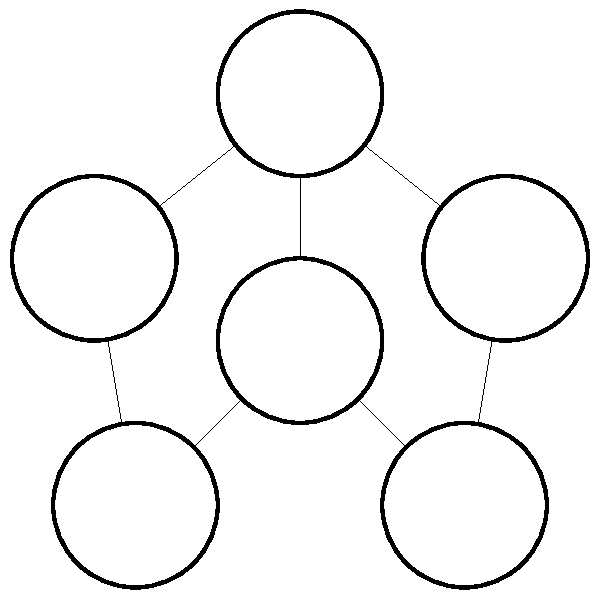
\includegraphics[scale=0.4]{images/Graph_2_Faerben}	
	\end{center}
\end{frame}
\begin{frame}
	\frametitle{Beispiel Graph-Färbbarkeit}
	\textbf{Ist dieser Graph 3-Färbbar?}
	\begin{center}
	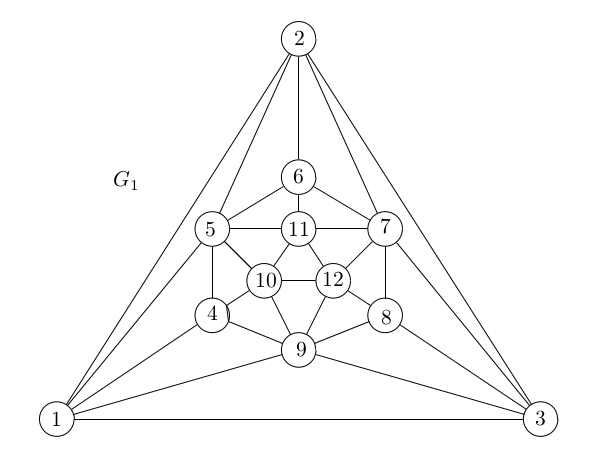
\includegraphics[scale=0.4]{images/4_Faerben}	
	\end{center}
\end{frame}

\subsection{Aufgabe B8 A3}
\begin{frame}
	\frametitle{Aufgabe zu Graphfärbbarkeit (B8 A3)}
	Gegeben seien ein ungerichteter Graph $G = (V,E)$ mit Knoten $v \in V$ und
	Kanten $e = (v_1,v_2) \in E$ mit $v_1, v_2 \in V$\\ und zwei Farben $A$ und $B$.\\
	Beweisen Sie: Die Sprache $\mbox{2-COLOR} \; =$\\
	$\{G \; | \; G = (V,E) \; \mbox{ungerichteter Graph mit} \; \exists \; \mbox{totale
	Funktion} \; g: V \to \{A,B\}: \forall \; (v_1, v_2) \in E: g(v_1) \neq g(v_2)\}$\\
	liegt in der Komplexit"atsklasse \textbf{P}.
\end{frame}

\section{2-SAT}
\subsection{Erkläung}
\begin{frame}
	\frametitle{n-SAT}
	\begin{block}{Kurzdefinition}
	Das selbe wie SAT allerdings enthalten ALLE Klauseln exakt n Literale enthält.\\
	\end{block}
	\begin{block}{Formal}
\textbf{Gegeben:} Formel in konjunktiver Normalform
\begin{itemize}
 \item Menge $U$ von Variablen
 \item Menge $C$ von Klauseln (Disjunktionen) über $U$ mit je exakt n Literalen
\end{itemize} %$$ \underbrace{(\stackrel{\text{Literale}}{\stackrel{\downarrow}{\vphantom{\neglit{a}}a} \vee \stackrel{\downarrow}{\vphantom{\neglit{b}}b} \vee \stackrel{\downarrow}{\neglit{c}}})}_\text{Klausel} \wedge \underbrace{(b \vee c)}_\text{Klausel} \wedge \underbrace{(\neglit{a} \vee \neglit{b} \vee \neglit{c})}_\text{Klausel}$$

\textbf{Frage:} Existiert eine (alle Klauseln) erfüllende Variablenbelegung?
\end{block}

\end{frame}
\subsection{Beispiel}
\begin{frame}
	\frametitle{Beispiele}
	\textbf{3-Sat}
	\[U=\{ a,b,c,d \}\]
	\[C=\{\{\neg a,\neg b,d\},\{\neg b,\neg a,c\},\{\neg c,\neg d, a\},\{b,c,d\}\}\]
	\textbf{2-Sat}
	\[U=\{ a,b,c,d,e \}\]
	\[C=\{\{a,\neg b\},\{\neg b,\neg d\},\{b,\neg d\},\{\neg c,d\},\{d,e\},\{d,\neg e\}\}\]
\end{frame}

\section{Weitere Aufgaben}
\subsection{2-COLOR auf 2-SAT Reduktion (B8 A4)}
\begin{frame}
	\frametitle{Reduktionsaufgabe (B8 A4)}
	Das Problem 2-SAT ist folgenderma"sen definiert:\\
	\begin{figure}[ht]
	\setbox0\vbox{\small
	\textbf{2-SAT}\\
	Gegeben eine in ihrer Gr"o"se polynomiell beschr"ankte aussagenlogische Formel $F$
	in konjuktiver Normalform, wobei jede Klausel genau 2 Literale enth"alt. $F$ hat
	also die Form
	\begin{eqnarray*}F = \Lambda_{i = 1}^n (L_i \vee N_i),\end{eqnarray*}
	wobei $L_i$ und $N_i$ Literale sind, also von der Form $X$ oder $\neg X$ f"ur eine
	Variable $X$ sind.\\
	Gibt es eine erfüllende Belegung für $F$?
	}
	\centerline{\fbox{\box0}}
	\end{figure}
	Geben Sie eine polynomielle Reduktion von 2-COLOR auf 2-SAT an!
\end{frame}
\subsection{B8 A1}
\begin{frame}
	\frametitle{Aufgabe B8 A1}
	\only<1>{
	Ein Algorithmus, der eine Zahl $n \in \mathbb{N}$ als Eingabe erh"alt und pr"uft,
	ob $n$ prim ist, sei gegeben durch die\\
	nachfolgende Beschreibung einer Turingmaschine $\mathcal{M}$, die die Funktion
	$f: \mathbb{N} \to \{0,1\}, n \mapsto
	\left\{\begin{array}{c@{\hspace{0.2cm},\hspace{0.2cm}}l}
	1 & n \; \mbox{prim}\\0 & \mbox{sonst}
	\end{array}\right.$\\
	realisiert.\\[4pt]}
	\only<2>{
	1. Initialisiere Z"ahler $z$ mit $2$ und Ausgabe $a$ mit $1$\\
	2. Berechne $n \; \% \; z$\\
	3. Pr"ufe, ob $n \; \% \; z = 0$ gilt:\\
	- Falls ja: Setze $a$ auf $0$ und gehe zu Schritt 4.\\
	- Falls nein: Gehe zu Schritt 4.\\
	4. Pr"ufe, ob $z < n$ gilt:\\
	- Falls ja: Erh"ohe $z$ um $1$ und gehe zu Schritt 2.\\
	- Falls nein: L"osche das Band, schreibe $a$ auf das Band und stoppe\\[4pt]
	Geben Sie die Komplexit"at des oben angegebenen Algortihmus bez"uglich der Eingabe
	$n$ und auch bez"uglich der\\
	L"ange der Bin"ardarstellung von $n$ an!}
\end{frame}

\section{Schluss}
\subsection{Schluss}
\begin{frame}
\frametitle{Bis zum nächsten Mal!}
\begin{center}
	%TODO: Aktuellen Comic einfügen
	
\includegraphics[width=1 \textheight]{images/xkcd_981.png}
\end{center}
\end{frame}

\frame{
  \frametitle{Lizenzen}
  \center
  
\includegraphics[width=2em]{images/by}
  
\includegraphics[width=2em]{images/cc}
  
\includegraphics[width=2em]{images/sa}
  \\
  {\tiny

Dieses Werk ist unter einem ``Creative Commons Namensnennung-Weitergabe unter gleichen Bedingungen 3.0 Deutschland``-Lizenzvertrag lizenziert. Um eine Kopie der Lizenz zu erhalten, gehen Sie bitte zu \href{http://creativecommons.org/licenses/by-sa/3.0/de/}{http://creativecommons.org/licenses/by-sa/3.0/de/} oder schreiben Sie an Creative Commons, 171 Second Street, Suite 300, San Francisco, California 94105, USA.\\
  \vspace{1cm}
  Davon ausgenommen sind das Titelbild, welches aus der März-April 2002 Ausgabe von American Scientist erschienen ist und ohne Erlaubnis verwendet wird, sowie das KIT Beamer Theme. Hierfür gelten die Bestimmungen der jeweiligen Urheber.
  \vspace{1cm}
  \\ 
  }
  %Habe hier die Reihenfolge etwas umgestellt, weil die Formatierung bei mir komisch aussah. 
  %Wenn es bei dir anders ist, kannst du es auch wieder zurückändern, dann haben wir unterschiedliche Kompilieroptionen
}

\end{document}